% AUTO-GENERATED by scripts/make_dose_response_pgf.py — do not edit.
% Data: LGES/vla_training/probes/0729_state_*_ramp{8,10,12}.txt, ALL-frames row.
\definecolor{figcond}{HTML}{0072B2}
\definecolor{fignaive}{HTML}{D55E00}
\definecolor{figkept}{HTML}{CC79A7}
\definecolor{figshuf}{HTML}{009E73}
\definecolor{figmuted}{HTML}{767676}
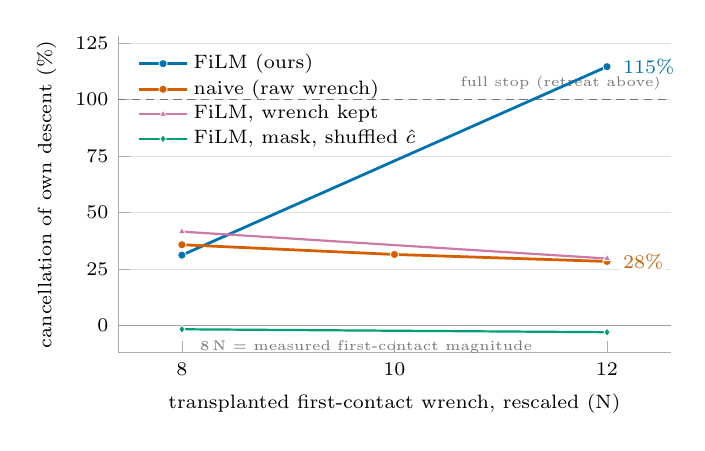
\begin{tikzpicture}
\begin{axis}[
  width=8.6cm, height=5.6cm, xmin=7.4, xmax=12.6, xtick={8,10,12},
  ymin=-12, ymax=128, ytick={0,25,50,75,100,125},
  xlabel={transplanted first-contact wrench, rescaled (N)},
  ylabel={cancellation of own descent (\%)},
  tick label style={font=\scriptsize}, label style={font=\scriptsize},
  axis x line*=bottom, axis y line*=left,
  axis line style={figmuted!60, line width=0.4pt},
  tick style={figmuted!60},
  ymajorgrids, grid style={figmuted!22, line width=0.3pt},
  clip=false, legend style={draw=none, fill=none, font=\scriptsize,
    legend cell align=left, at={(0.02,0.98)}, anchor=north west, row sep=-1.5pt},
]
\addplot[figmuted, dash pattern=on 3pt off 2pt, line width=0.5pt, forget plot] coordinates {(7.4,100) (12.6,100)};
\node[font=\tiny, figmuted, anchor=south east] at (axis cs:12.6,100) {full stop (retreat above)};
\addplot[figmuted!70, line width=0.4pt, forget plot] coordinates {(7.4,0) (12.6,0)};
\node[font=\tiny, figmuted, anchor=west] at (axis cs:8.08,-9.5) {8\,N = measured first-contact magnitude};
\addplot[figcond, solid, line width=1.0pt, mark=*, mark size=1.5pt, mark options={solid, fill=figcond, draw=white, line width=0.3pt}] coordinates {(8,31.2) (12,114.6)};
\addlegendentry{FiLM (ours)}
\node[font=\scriptsize, figcond, anchor=west, fill=white, inner sep=1pt] at (axis cs:12.12,114.6) {$115\%$};
\addplot[fignaive, solid, line width=1.0pt, mark=*, mark size=1.5pt, mark options={solid, fill=fignaive, draw=white, line width=0.3pt}] coordinates {(8,35.8) (10,31.5) (12,28.4)};
\addlegendentry{naive (raw wrench)}
\node[font=\scriptsize, fignaive, anchor=west, fill=white, inner sep=1pt] at (axis cs:12.12,28.4) {$28\%$};
\addplot[figkept, solid, line width=0.8pt, mark=triangle*, mark size=1.5pt, mark options={solid, fill=figkept, draw=white, line width=0.3pt}] coordinates {(8,41.6) (12,29.7)};
\addlegendentry{FiLM, wrench kept}
\addplot[figshuf, solid, line width=0.8pt, mark=diamond*, mark size=1.5pt, mark options={solid, fill=figshuf, draw=white, line width=0.3pt}] coordinates {(8,-1.6) (12,-2.9)};
\addlegendentry{FiLM, mask, shuffled $\hat{c}$}
\end{axis}
\end{tikzpicture}
